
\begin{figure}[H]
  \centering
  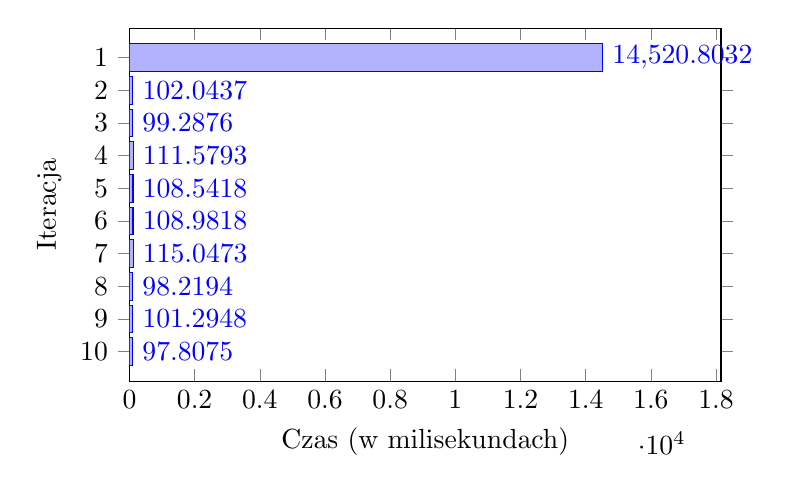
\begin{tikzpicture}
  
    \begin{axis} [
      xbar = .05cm,
      nodes near coords,
      nodes near coords style={
        /pgf/number format/precision=4,
      },
      xmin = 0,
      ytick = data,
      enlarge x limits = {value = .25, upper},
      symbolic y coords = {10,9,8,7,6,5,4,3,2,1},
      xlabel=Czas (w milisekundach),
      ylabel=Iteracja,
      width=0.75\textwidth,
      height=0.5\textwidth
    ]
    
      \addplot coordinates {(14520.803200006485,1) (102.04370003938675,2) (99.28759998083115,3) (111.57929998636246,4) (108.5417999625206,5) (108.98179996013641,6) (115.04729998111725,7) (98.21939998865128,8) (101.29479998350143,9) (97.80750000476837,10)};
      
    \end{axis}
  
  \end{tikzpicture}
  \caption{Wynik testów przykładu 5 [\ref{lst:wydajnosc-przyklad-p-5}]}
  \label{fig:wynik-przyklad-4}
\end{figure}
